\section{Signal simulation}
\label{sec:signalsim}
In  this section, we  describe briefly  the detector  simulation. More
details   on    this   study   can    be   found   in    a   separated
note~\cite{noteelec}. Here, we only deal with the detector simulation,
we  assume that  we  know the  power  received (the  signal after  the
antenna).
\subsection{Detector simulation}
The skeleton  of an EASIER detector  is the same for  all the versions
:EASIER/GIGADuck  C-band,  GIGADuck  Helix.   It  is  composed  of  an
antenna,  an amplification  stage,  a power  detection, an  adaptation
stage and finally the SD FADC.  To simulate a realistic radio trace we
simulate  these stages  one by  one. We  first simulate  an  RF (radio
frequency)  waveform according  to the  receiver's bandwidth.  This RF
waveform  is  then processed  by  the  power  detector and  the  board
response. Finally  we sample  this waveform in  time and  amplitude to
obtain  a trace we  can compare  to actual  data. We  sum up  here the
methods used to simulate these parts:
\begin{itemize}
\item \textbf{antenna + LNA:} The antenna and LNA (or LNB) association
  is  the RF  (radio frequency)  part, it  sets the  bandwidth  of the
  receiver.  The  spectrum of the association  antenna+LNA(or LNB) was
  measured  for  all   the  detector  types  and  are   shown  in  the
  figure~\ref{fig:spectra}. From  the spectrum and an  random phase, a
  RF  waveform is  generated by  inverse  FFT.  The  amplitude of  the
  waveform is set according to the system noise temperature.
  \begin{figure}[H]                                                             
    \centering                                                                    
    \hspace*{-3ex}                                                                
    \subfigure{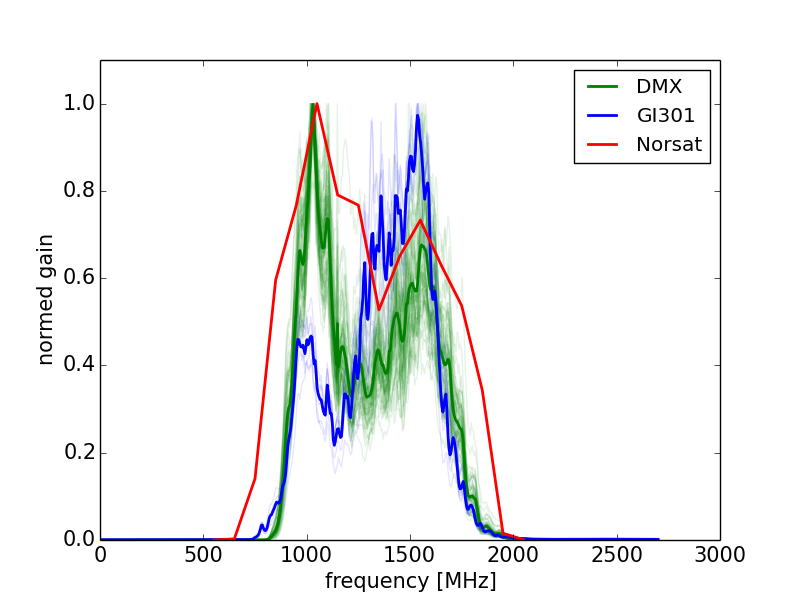
\includegraphics[width=0.49\linewidth]{spectra3.png}}        
    \caption{gain spectra for the three types of LNB in the C-band.}
  \label{fig:spectra}
  \end{figure}
\item \textbf{power detection:} the power detector output is simulated
  by  a  convolution of  an  exponential  decay  function and  the  RF
  waveform in  dBm unit.  The  parameters of the  exponential function
  were  deduced from lab  measurements.  In  the figure~\ref{fig:m3ex}
  (left) we  show an  example of the  measured RF waveform  (top), the
  power detector response (measured in  blue and simulated in red) and
  the difference for this particular waveform (bottom). The difference
  between measured  and simulated for a  set of waveforms  is shown in
  the  figure~\ref{fig:m3ex}   (right)  for  a   power  detector  with
  capacitor (in green) and without (in blue).
\begin{figure}[H]
  \centering
  \hspace*{-3ex}
  \subfigure{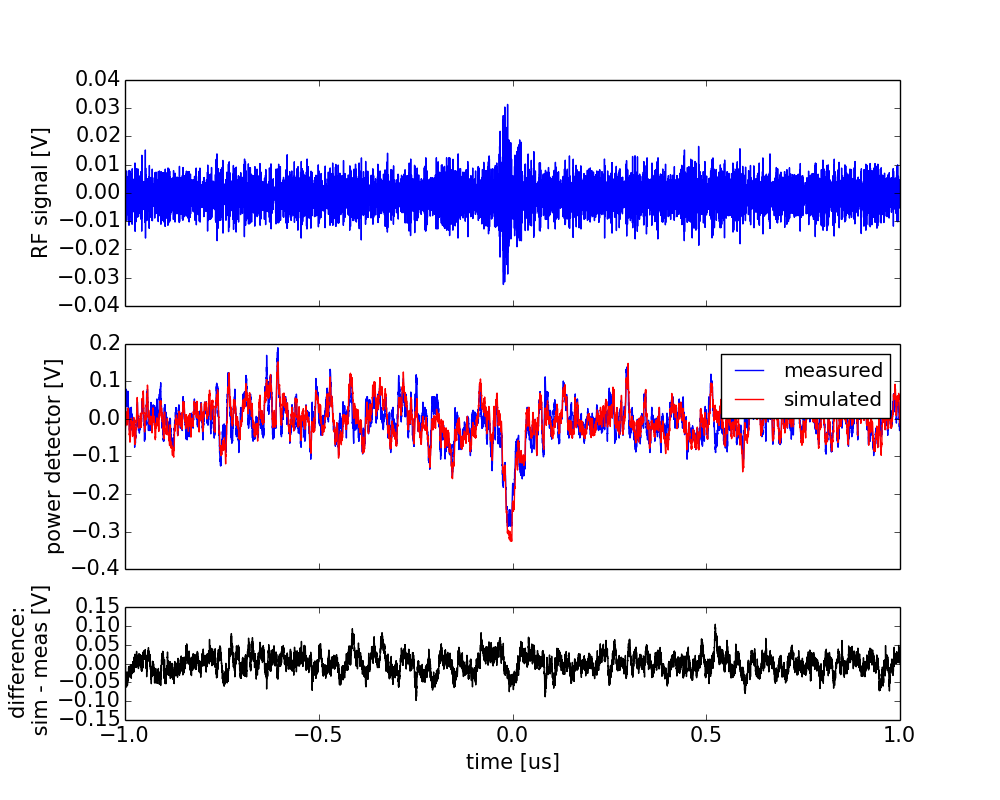
\includegraphics[width=0.49\linewidth]{nocapa_method3.png}}
  \subfigure{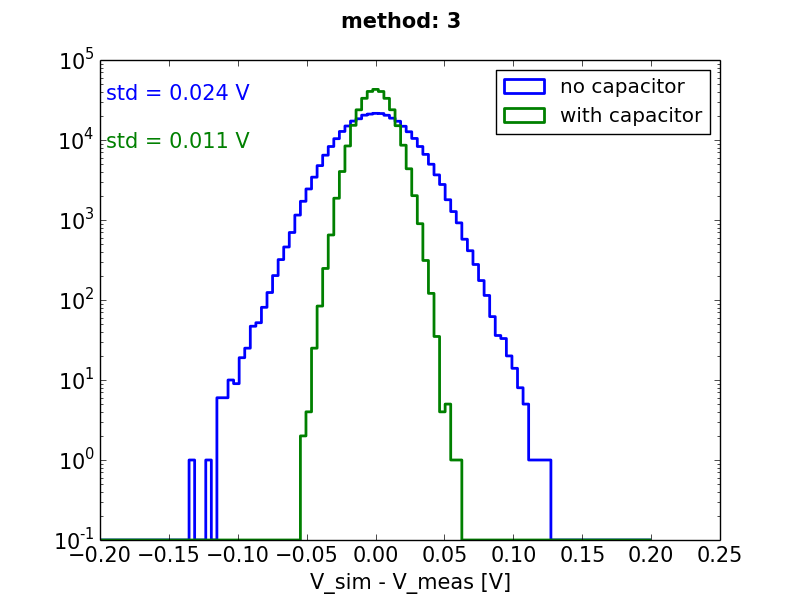
\includegraphics[width=0.49\linewidth]{res_method3.png}}
  \caption{power detector  simulation. left: superposition  of measured
    and simulated. right: distribution of the difference measured-simulated.}
  \label{fig:m3ex}
\end{figure}
\item  \textbf{adaptation  stage:}  this  stage  amplifies  the  power
  detector output in order to  adjust the dynamic range.  The stage is
  simulated with the transfer function  measured in lab. The gain as a
  function  of  the frequency  for  this  amplifier  is shown  in  the
  figure~\ref{fig:board} (left)  and an  example of simulation  in the
  figure~\ref{fig:board} (right)
\begin{figure}[H]
  \centering
  \hspace*{-3ex}
  \subfigure{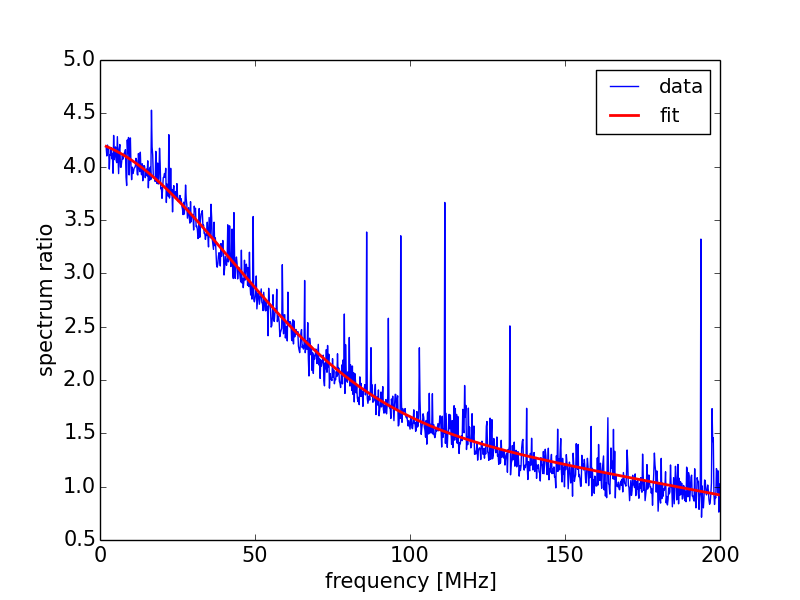
\includegraphics[width=0.45\linewidth]{fitspecboard.png}}
  \subfigure{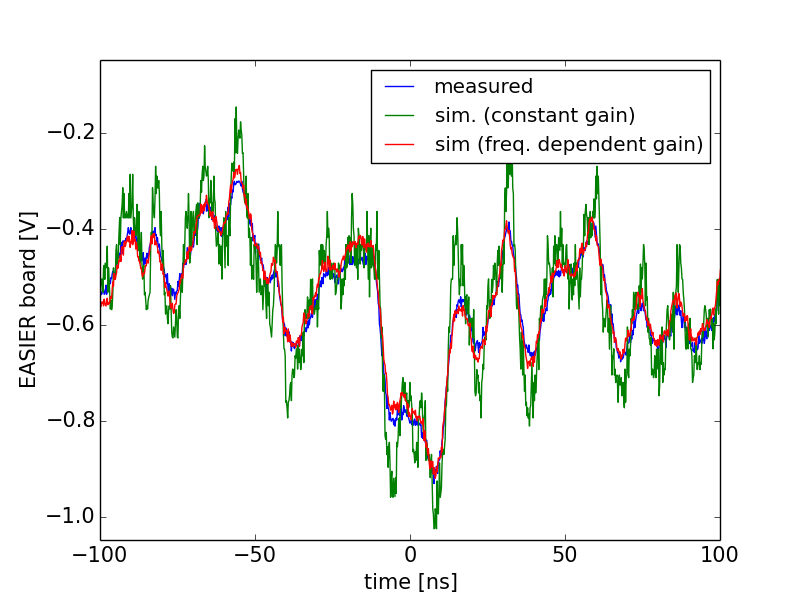
\includegraphics[width=0.45\linewidth]{examplesimboard.png}}
  \caption{left: the board transfer  function. right: example of board
    simulation, in green  the board is simulated with  a constant gain
    (simple  linear  relation  between  the  power  detector  and  the
    board.),  in  red it  is  simulated  using  the measured  transfer
    function.}
  \label{fig:board}
\end{figure}
\item \textbf{SD FADC:}  The input of the Auger SD  front end has anti
  aliasing filter. It is simulated  with a 4$\rm ^{th}$ order low pass
  filter with a cut frequency of 20 MHz. The signal is then sampled in
  time at 40MSamples/s and in amplitude over 1024 ADC counts on 1V.
\end{itemize}
The  comparison  of   the  simulation  with  data  is   shown  in  the
figure~\ref{fig:compsimdata}. It shows  the distribution in ADC counts
of the measured and simulated traces (after baseline subtraction).
\begin{figure}[!ht]
  \centering
  \hspace*{-3ex}
  \subfigure{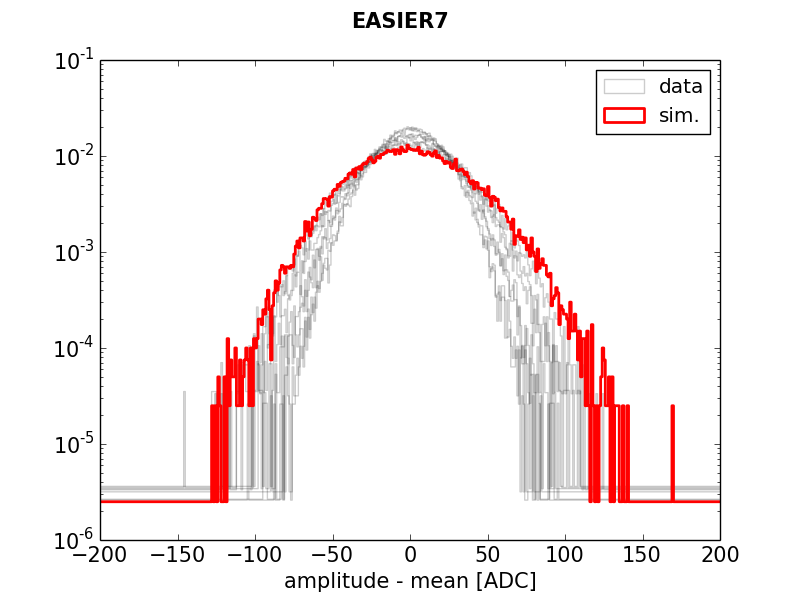
\includegraphics[width=0.32\linewidth]{m3_distdatasimEA7.png}}
  \subfigure{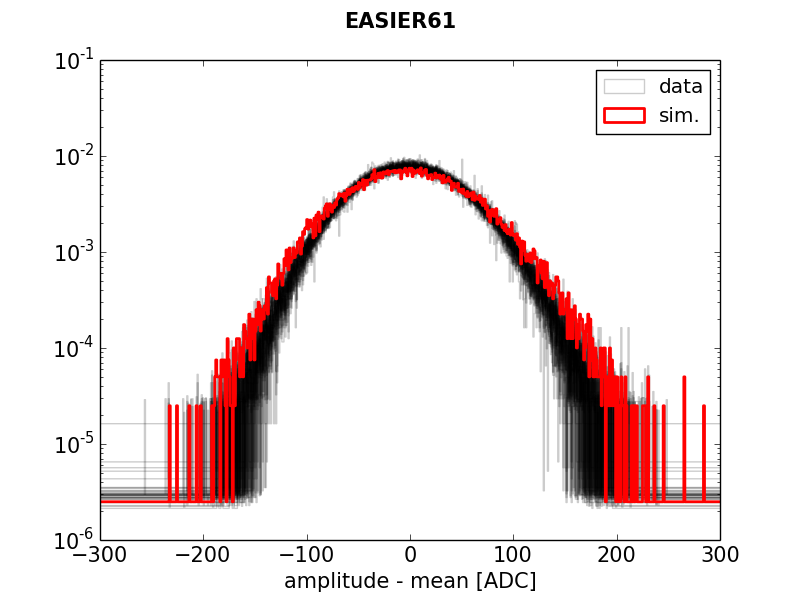
\includegraphics[width=0.32\linewidth]{m3_distdatasimEA61.png}}
  \subfigure{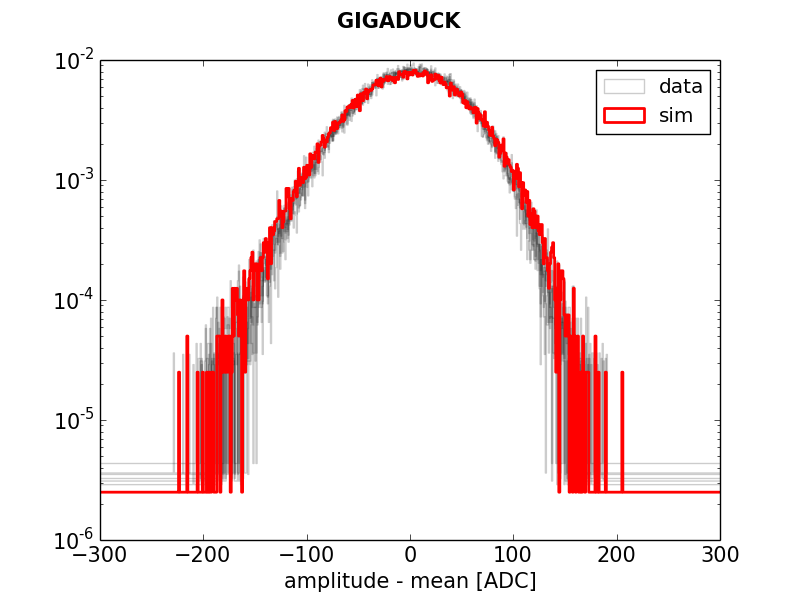
\includegraphics[width=0.32\linewidth]{m3_distdatasimGD.png}}
  \caption{comparison of the measured distribution of amplitude and the simulated one.}
  \label{fig:compsimdata}
\end{figure}
In  the simulation described  above, we  haven't mentioned  the system
noise temperature or  the absolute gain of the  system.  In fact these
parameters will  only change the  value of the average  baseline, they
won't change the RMS.
\subsection{Signal simulation}
The  RF   noise  is  simulated   according  to  the  spectra   of  the
figure~\ref{fig:spectra} and the absolute noise level is given by:
\begin{equation}
  \rm  P_{noise} = k_B T_{sys} \Delta \nu 
\end{equation}
where  $\rm  \Delta  \nu$  is  the  bandwidth  (i.e.   the  normalized
integrated power cf~\cite{noteelec}).\\The  signal is generated with a
power envelope, an example of  a gaussian envelope is presented in the
fig~\ref{fig:exsignal}  (left).  To  obtain  a RF  signal waveform  we
generate another normalized  noise waveform and we multiply  it by the
amplitude envelope. The results is shown in the fig~\ref{fig:exsignal}
(middle).  When  added to the noise,  we obtain the  waveform shown in
the  fig~\ref{fig:exsignal}  (right).\\   This  RF  waveform  is  then
processed according to the electronics simulation described before.
\begin{figure}[!ht]
  \centering
  \hspace*{-3ex}
  \subfigure{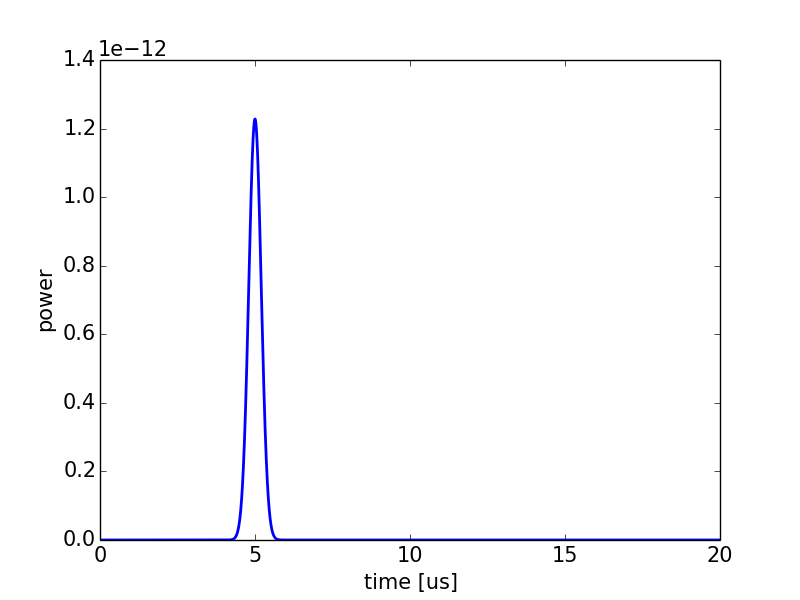
\includegraphics[width=0.32\linewidth]{exsigenv.png}}
  \subfigure{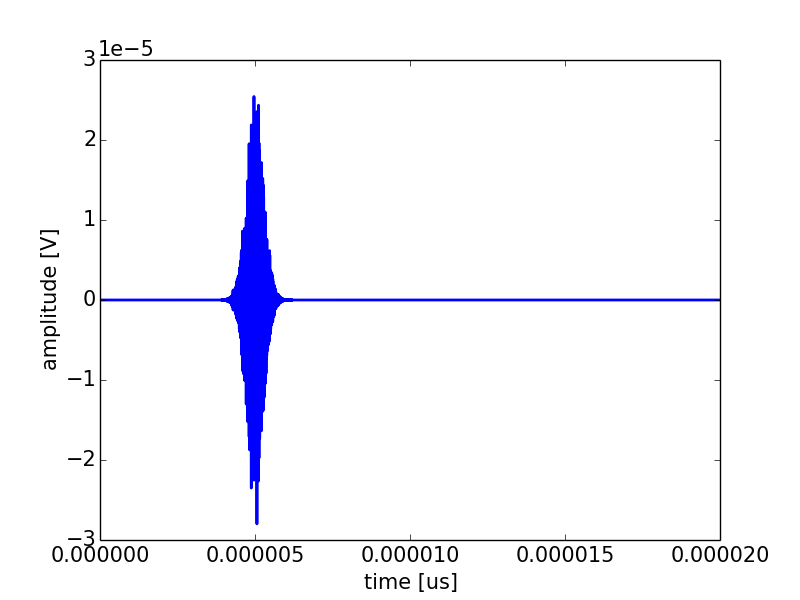
\includegraphics[width=0.32\linewidth]{exsigamp.png}}
  \subfigure{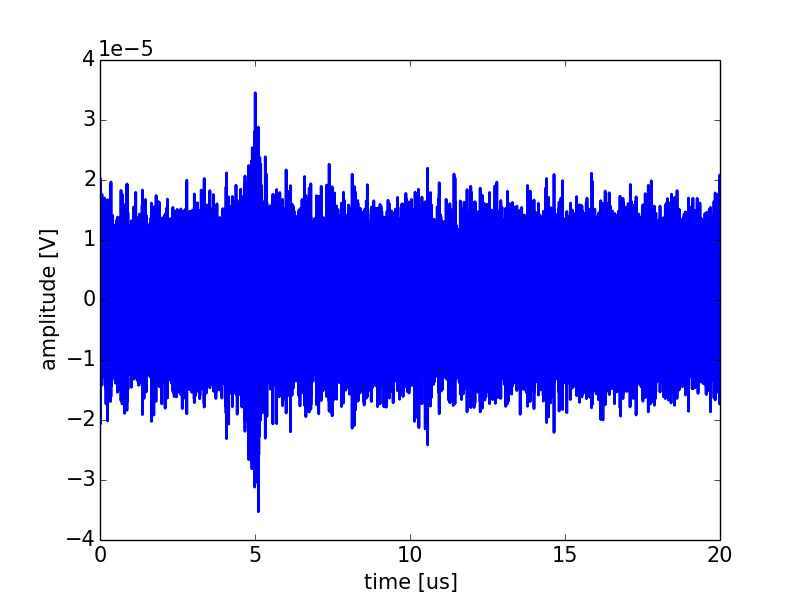
\includegraphics[width=0.32\linewidth]{exnoisesigenv.png}}
  \caption{steps of the RF waveform simulation}
  \label{fig:exsignal}
\end{figure}


\subsection{Power estimate}
We described the  signal simulation in the previous  paragraph. Now we
are able to simulate a EASIER trace signal from a RF trace. We want to
know if we  can actually come back to the input  power with the EASIER
trace.\\ We  produce a set of  simulation with a  Gaussian envelope as
input  signal with an  SNR varying  from 1  to 10  and the  width from
\unit[10]{ns} to  \unit[500]{ns}.  To estimate the  power, we multiply
the  ADC   waveform  with  the   board  and  the  power   detector  DC
characteristics  (that  mean  we   don't  account  for  any  frequency
dependence).  This gives us the  estimated power in dBm, so finally we
convert this  power in Watt.  The  output SNR is found  by fitting the
retrieved power trace, see for example the figure~\ref{fig:exfit}, and
the   comparison  of   input  and   output   SNR  is   shown  in   the
figure~\ref{fig:estimate}.  For  very short signal  (10ns), the output
SNR is underestimated because of  the filtering of the power detector,
this is clear  when comparing the results in the  case we simulate the
power  detector with  capacitor or  without. The  case  with capacitor
filters at  lower frequencies  and cuts more  the short  signals.  For
longer signal the output SNR is slightly overestimated by 10 to 15 \%.
I still  don't understand the reason  but the study  presented in this
note will  compare methods to  improve the SNR  it is not  critical to
have a systematic bias.
\begin{figure}[!ht]
  \centering
  \hspace*{-3ex}
  \subfigure{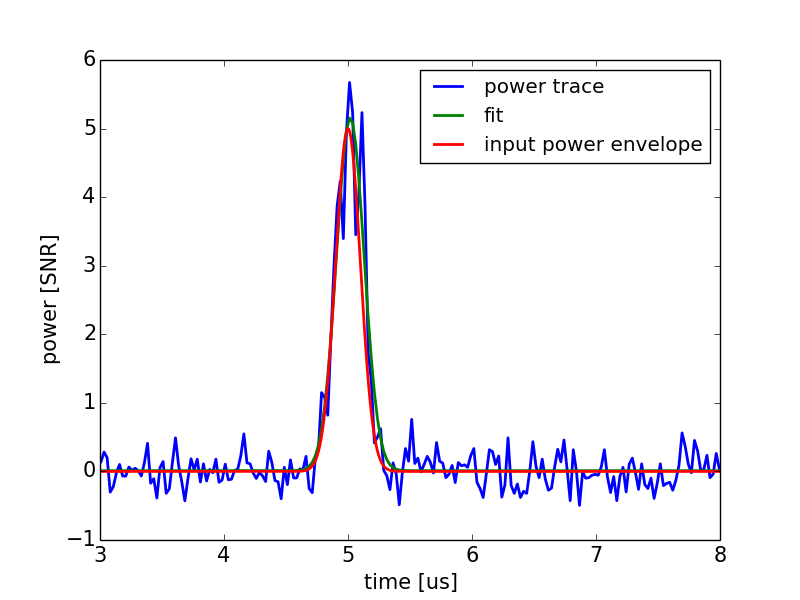
\includegraphics[width=0.45\linewidth]{examplepowerestimatenorsat.png}}
  \subfigure{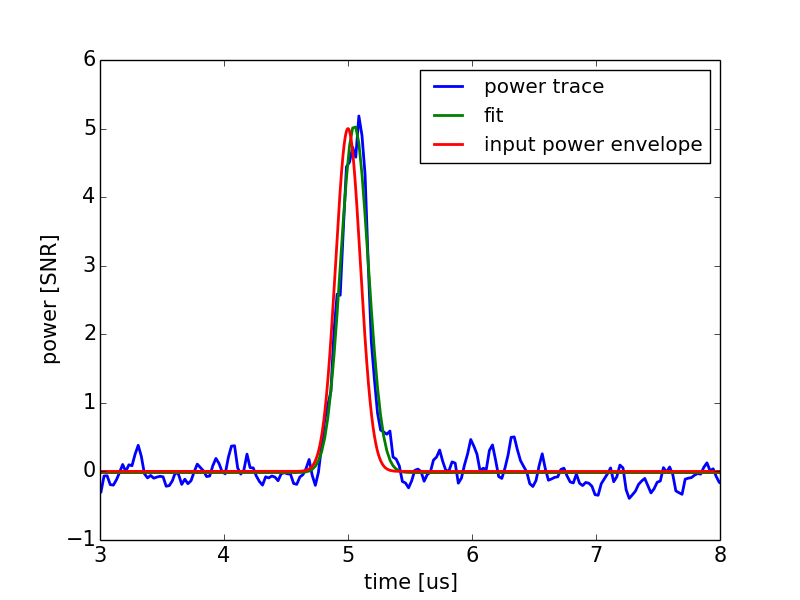
\includegraphics[width=0.45\linewidth]{examplepowerestimate.png}}
  \caption{Output  after detector  simulation  and back  to power.  In
    green the gaussian fit and in  red the input. Left: for Norsat and
    no capacitor case. Right: for GI antenna and with capacitor case.}
  \label{fig:exfit}
\end{figure}
\begin{figure}[!ht]
  \centering
  \hspace*{-3ex}
  \subfigure{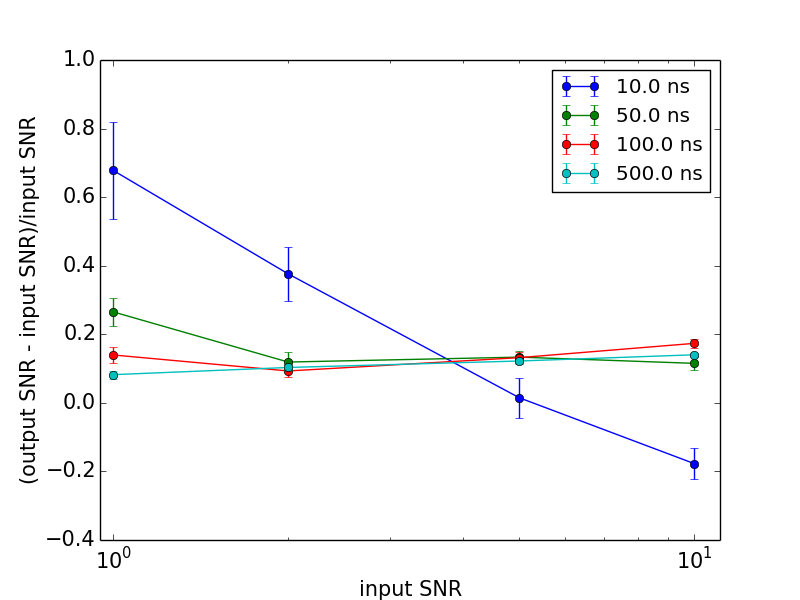
\includegraphics[width=0.45\linewidth]{powerestimatenorsat.png}}
  \subfigure{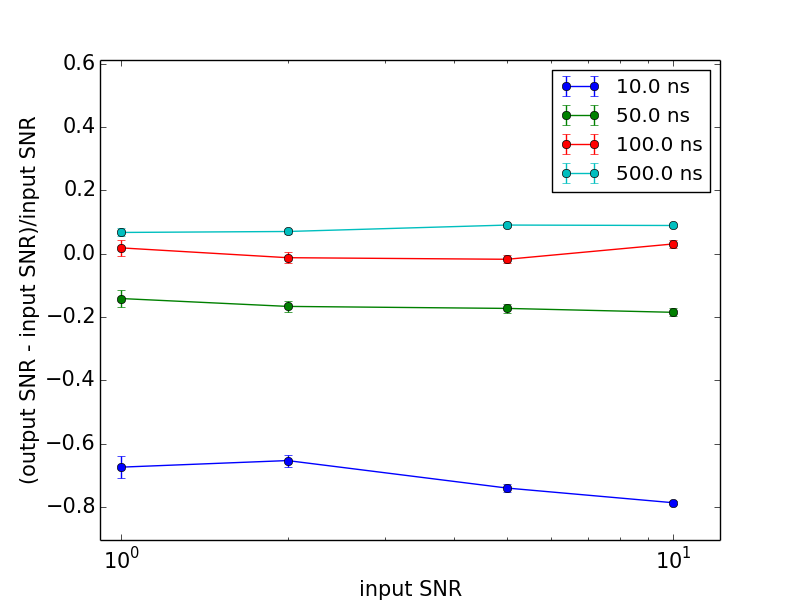
\includegraphics[width=0.45\linewidth]{powerestimategi.png}}
  \caption{comparison  of   input  and  output   SNR  (after  detector
    simulation and back  to power). Left: for Norsat  and no capacitor
    case. Right: for GI antenna and with capacitor case.}
  \label{fig:estimate}
\end{figure}


